% !TEX program = lualatex
% !TEX format = pdf
% !TEX encoding = UTF-8

\documentclass[phdthesis,12pt,final]{wuthesis}

\usepackage{ifluatex}
\ifluatex
  \usepackage{fontspec} % international characters

  \usepackage{polyglossia}
  \setmainlanguage[variant=american]{english}
\else % use for pdflatex
  \usepackage[utf8]{inputenc}
  \usepackage[T1]{fontenc}

  \usepackage[USenglish]{babel}
\fi

\usepackage{microtype} % typographical perfection
\usepackage{csquotes}
\usepackage[vskip=0pt,begintext=\textooquote,endtext=\textcoquote]{quoting}
\SetBlockEnvironment{quoting}

\usepackage[
  backend=biber,
  isbn=false,
  url=false,
  sortcites,
  maxbibnames=8
]{biblatex}
\addbibresource{references.bib}

\usepackage{amsmath}
\usepackage{amsfonts}

\usepackage[section]{placeins} % stop floats at sections
\usepackage[inline, shortlabels]{enumitem}
\usepackage{threeparttable}
\usepackage{booktabs}
\usepackage{array}
\usepackage{siunitx}
\usepackage{makecell}
\newcommand{\stretchtable}[1][1.4]{\renewcommand{\arraystretch}{#1}}
\usepackage{mdframed}

% use links in document. load last.
\usepackage[hidelinks,linktoc=all]{hyperref}
\usepackage[noabbrev]{cleveref}
\newcommand{\crefrangeconjunction}{--}
\usepackage{caption}

%%%%%%%%%%%%%%%%%%%%%%%%%%%%%%%%%%%%%%%%%%%%%%%%%%%%%%%%%%%%%%%%%%%%%%%%%%%%%
%%
%% These commands customize the `wuthesis' package for me
%%
%%%%%%%%%%%%%%%%%%%%%%%%%%%%%%%%%%%%%%%%%%%%%%%%%%%%%%%%%%%%%%%%%%%%%%%%%%%%%

%% Enter your official name
\renewcommand{\thesisauthor}{Paige Turner}
\renewcommand{\thesisauthorlastname}{Turner}

%% Enter your previous degrees
%% If you have no previous degrees remember to remove the comma too.
%\renewcommand{\thesisauthorpreviousdegrees}{, J.D.}

%% Enter department name
\renewcommand{\thesisdepartment}{Department of Computer Science and Engineering}
\renewcommand{\thesisfield}{Computer Science}

%% Enter date of graduation
\renewcommand{\thesismonth}{May}
\renewcommand{\thesisyear}{2016}

%% Enter title of thesis
\renewcommand{\thesistitle}{A Mock Thesis on the Proper Formatting of Dissertations and Theses for \\ Arts \& Sciences Graduate Students}

%% Enter the copyright holder ( DEFAULT is \thesisauthor )
%\renewcommand{\thesiscopyrightholder}{\thesisauthor}

%% Enter supervisor name
\renewcommand{\thesissupervisor}{Professor Katherine Davidsen, Chair\\
Professor Michael Randolf, Co-Chair}
%%
% list in alphabetical order
%%
\renewcommand{\thesiscommittee}{Katherine Davidsen, Chair\\
Michael Randolf, Co-Chair \\
Richard Lewis \\
Hillary O'Connell \\
Jack Taylor}

\renewcommand{\thesisdedication}{Dedicated to my parents.}

\hypersetup{
  pdftitle={\thesistitle},
  pdfauthor={\thesisauthor},
  pdfpagemode=UseOutlines,
  bookmarksnumbered=true,
  bookmarksopen=true,
  bookmarksopenlevel=1
}
\IfFileExists{upquote.sty}{\usepackage{upquote}}{}

\begin{document}

\frontmatter

% NOTE: do not put any text in the thesistitlepage, thesiscopyrightpage,
% or thesisdedicationpage sections.  If you want to use these pages, then you
% should remove the notes below (e.g., by uncommenting the \iffalse
% and \fi lines) and change the appropriate fields in thesis-main.tex.
% This will ensure that the copyright and dedication lines are positioned
% and formatted correctly.  Additionally, remove the
% thesisacknowledgmentpostscript and listoftablespostscript sections, since
% these are used to add explanatory notes which shouldn't be there in normal
% theses.

\begin{thesistitlepage}
\end{thesistitlepage}

\begin{thesiscopyrightpage}
\end{thesiscopyrightpage}

\begin{singlespace}
\setcounter{page}{2}
\renewcommand*\contentsname{Table of Contents}
\tableofcontents

% If one or more figures are used in the document, there must be a list of all figures and it must
% be included in the table of contents. The list should be spaced at 1.15. Begin each listing on a
% new line.
\cleardoublepage
\phantomsection
\addcontentsline{toc}{chapter}{\listfigurename}
\listoffigures

% If one or more tables are used in the document, there must be a list of all tables and it must be
% included in the table of contents. The list should be spaced at 1.15. Begin each listing on a new
% line.
\cleardoublepage
\phantomsection
\addcontentsline{toc}{chapter}{\listtablename}
\listoftables
\end{singlespace}

\begin{thesisacknowledgments}
An acknowledgments page must be included in your final dissertation or thesis.
If you wish to include a special dedication you can either use it to close the acknowledgments page or place it on the page that immediately follows.
The acknowledgments page should be listed in the table of contents.
Place it after the final list used in the document, and before any dedication, abstract, or epigraph that is included.

It is appropriate to acknowledge sources of academic and financial support; some fellowships and grants require acknowledgment.

We offer special thanks to the Washington University School of Engineering for allowing us to use their dissertation and thesis template as a starting point for the development of this document.
\end{thesisacknowledgments}

% Note: If you include a special dedication as shown here be sure to keep it brief and center it on
% the page both horizontally and vertically. Alternatively, you may remove this page altogether,
% and a special dedication can be placed as the final paragraph of your acknowledgments page. Do
% not include the dedication page in your table of contents.
\begin{thesisdedicationpage}\label{dedication}
\end{thesisdedicationpage}

\cleardoublepage
\phantomsection
\begin{thesisabstract}
After removing these comments, begin typing the body of your abstract here, double-spaced.
Your font should be 12-point (which is the text of this sample paragraph).
No part of the abstract should be bolded.
If this is for your master's degree, be sure to change all occurrences of the word ``dissertation'' to display as ``thesis,'' and change ``Doctor of Philosophy'' or ``Doctor of Liberal Arts'' to ``Master of Arts,'' ``Master of Liberal Arts,'' or ``Master of Fine Arts,'' whichever applies.
In the abstract heading above, make sure you use the year your degree is to be officially earned.
Be sure to use your full name as it is recorded in WebSTAC, your dissertation or thesis advisor's full name(s) wherever appropriate, and the correct title of your degree whenever referencing it.
The title of your degree will not always be the same as the title of your department or program, so please check with your departmental administrative assistant and adviser(s) to be sure you are using the correct degree title.
Please note that an abstract is required for all dissertation submissions in ProQuest.
An abstract is optional for master's thesis submissions.
\end{thesisabstract}

\mainmatter
% !TEX root = thesis.tex

\chapter{Introduction}
\label{ch:1}

Identifying the scene from which an image was captured is a problem of great interest in the computer vision community. Work in this area involves both classification tasks, where the goal is to identify the specific scene category (e.g., park, beach, church), as well as recognition tasks, where the goal is to identify the precise location where an image was captured. These tasks can be grouped based on the specificity of the categories~\cite{grauman_leibe_2011}:

\begin{enumerate}
    \item Basic-level categories (e.g., `building')
    \item Specialized categories (e.g., `church')
    \item Exact instances (e.g., `the Notre-Dame')
\end{enumerate}

The first task (``What is in this picture?'') is the basic level classification task. The second task (``What type of building is in this picture?'') can be referred to as \emph{\textbf{scene} recognition} and the third task (``What specific church is in this picture?'') as \emph{\textbf{place} recognition}.

Scene recognition requires learning the shared properties of the examples in the specialized class, while place recognition requires learning the specific components and their configuration that correspond to a particular instance.

Hotel recognition is the task of identifying what hotel is seen in a photograph. While this problem is similar to other scene and place recognition tasks, it has unique properties that make it a particularly challenging recognition problem: within a hotel, the rooms may have some objects that are the same (e.g., every room has the same headboard), some objects that are different (e.g., different artwork on the walls), and those objects may be in different configurations from room to room (e.g., two beds vs. one or furniture on different walls). Additionally, those same objects may be seen in different hotels from the same hotel chain around the world.

Hotel recognition does not fit neatly into either the scene recognition or the place recognition task. It requires learning both the general, shared properties of all of the rooms in a particular hotel, such as its decor or star rating or commonly used color profiles, as well as recognizing exact duplicated instances of furniture, art and bedding that may be used in different configurations throughout the hotel.

These differences from standard recognition problems necessitate novel datasets and deep learning approaches in order to successfully perform hotel recognition. In this dissertation, I will present my work in building these datasets, training deep convolutional networks on the task of hotel recognition, and generating visualization approaches that seek to identify what deep networks trained on image similarity and recognition problems are learning.

\section{The Importance of Hotel Recognition}
In addition to understanding the datasets and algorithms that are necessary to successfully perform hotel recognition, it is important to understand our particular motivation for working in this space.

In recent years, the number of images of victims of human trafficking shared online has grown at an alarming rate~\cite{bouche2015report,ncmecAmicusBrief}. Whether used for advertising or exchanged among criminal networks, these photographs serve as visual evidence of where the victim was trafficked.

Such images are often captured in hotel rooms. Identifying the hotels in these photographs gives insight into where a trafficking victim has been moved previously and where their trafficker may move them or others in the future. Understanding how traffickers operate, and how to rescue victims is a top priority for law enforcement~\cite{nationalStrategy}.

\begin{figure}
    \centering
    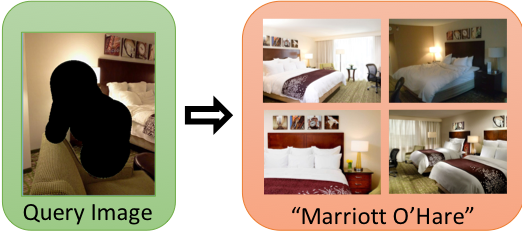
\includegraphics[width=.7\columnwidth]{figures/chapter1/victimQuery_to_hotel.png}
    \caption{The task of hotel recognition in cases of human trafficking involves identifying the particular hotel from an image of a trafficking victim.}
    \label{fig:victimQuery_to_hotel}
\end{figure}

Figure~\ref{fig:victimQuery_to_hotel} shows an example image from investigators, where a victim is posed in a hotel room. The hotel recognition task is to identify what hotel the victim was photographed in. The properties of the victim photographs further complicate the hotel recognition task -- the images are often of low quality, from uncommon camera perspectives, with large occlusions (often the victim).

Developing hotel recognition algorithms that are robust to these difficult query conditions is not only an interesting computer vision challenge, but also has very real human impacts.
% !TEX root = thesis.tex

\chapter{Understanding Hotel Recognition in the Context of Scene and Place Recognition}
\label{ch:2}

Identifying the scene from which an image was captured is a problem of great interest in the computer vision community. Work in this area involves both classification tasks, where the goal is to identify the specific scene category (e.g., park, beach, church), as well as recognition tasks, where the goal is to identify the precise location where an image was captured. These tasks can be grouped based on the specificity of the categories~\cite{grauman_leibe_2011}:

\begin{enumerate}
    \item Basic-level categories (e.g., `building')
    \item Specialized categories (e.g., `church')
    \item Exact instances (e.g., `the Notre-Dame')
\end{enumerate}

The first task (``What is in this picture?'') is the basic level classification task. The second task (``What type of building is in this picture?'') can be referred to as \emph{\textbf{scene} recognition} and the third task (``What specific church is in this picture?'') as \emph{\textbf{place} recognition}.

Scene recognition requires learning the shared properties of the examples in the specialized class, while place recognition requires learning the specific components and their configuration that correspond to a particular instance.

Hotel recognition, however, does not fit neatly into either the scene recognition or the place recognition task. It requires learning both the general, shared properties of all of the rooms in a particular hotel, such as its decor or star rating or commonly used color profiles, as well as recognizing exact duplicated instances of furniture, art and bedding that may be used in different configurations throughout the hotel.

% references
\begin{spacing}{1.0}
% Create References header for TOC
\defbibheading{references}[References]{%
\chapter*{#1}%
\addcontentsline{toc}{chapter}{#1}}

% Additional line break pass in references
\appto{\bibsetup}{\emergencystretch=1em}

\printbibliography[heading=references]
\end{spacing}
\clearpage

\appendix
% !TEX root = thesis.tex

\chapter[Degree Program]{What to Call your Degree Program on your Title Page and your Abstract Page}
\label{app:degree-program}

\paragraph{Title page}
The second line (or second and third lines) on the page must name your \emph{administrative unit}.

\begin{itemize}
\item If your degree is offered by one department of Arts \& Sciences on the Danforth Campus, your unit is that department: \\
\centerline{\emph{Department of East Asian Languages \& Cultures}}

\item For a co-sponsored degree such as English \& Comparative Literature, credit both: \\
\centerline{\emph{Department of English}}\\
\centerline{\emph{Program in Comparative Literature}}

\item For the Division of Biology \& Biomedical Sciences, credit DBBS and your program: \\
\centerline{\emph{Division of Biology \& Biomedical Sciences}}\\
\centerline{\emph{Neurosciences}}

\item Credit only the program for any of the non-DBBS PhDs on the Medical Campus: \\
\centerline{\emph{Interdisciplinary Program in Movement Science}}\\
\centerline{or}\\
\centerline{\emph{Program in Speech \& Hearing Sciences}}

\item If you are in a department in Engineering, credit the School and the department: \\
\centerline{\emph{School of Engineering \& Applied Science}}\\
\centerline{\emph{Department of Biomedical Engineering}}

\item If you are in social work or business, your administrative unit is the School: \\
\centerline{\emph{Brown School of Social Work}}\\
\centerline{or}\\
\centerline{\emph{Olin Business School}}
\end{itemize}

\paragraph{Abstract page}
Frequent confusion occurs because your abstract heading names your degree rather than your administrative unit, so it may – or may not – match your title page in that respect.

\begin{itemize}
\item For the Division of Biology \& Biomedical Sciences: \\
\centerline{\emph{Doctor of Philosophy in Biology and Biomedical Sciences}}\\
\centerline{\emph{Neurosciences}}

\item For a co-sponsored degree such as English \& Comparative Literature, credit both: \\
\centerline{\emph{Doctor of Philosophy in English and Comparative Literature}}

\item If you are in a department in Engineering, credit the School and the department: \\
\centerline{\emph{School of Engineering \& Applied Science}}\\
\centerline{\emph{Department of Biomedical Engineering}}

\item If your degree is offered by one department of Arts \& Sciences on the Danforth Campus: \\
\centerline{\emph{Doctor of Philosophy in Chemistry}}
\end{itemize}


\end{document}
